\subsection{RBC tumbling and tank-treading}

Few RBC models include viscoelastic forces. Fedosov \latin{et al.} use a particle-based
method to simulate the fluid and cells~\cite{Fedosov:2010bc}, where particles
representing the RBC membrane experience drag and random forces. Gounley and Peng use the
IB machinery to spread membrane viscosity to the fluid, thereby modifying the fluid
stress term~\cite{Gounley:2015ho}. Our intent in adding a viscoelastic response is to aid
in the numerical stability of the discrete RBCs. We wish to verify that the extended
model, with dissipative force, retains the ability to tumble and tank-tread, which is
commonly used to validate other RBC models~\cite{Yazdani:2011cl,Omori:2012hw,Fai:2013do,
Xu:2013kk}. To that end, we place a single RBC with $\data\cardinality=625$ and
$\sample\cardinality = 2500$ in the same domain as the previous section, now discretized
to have $h = 0.4\um$ and with moving top and bottom walls. In the interest of reducing
simulation time, we now use the backward-forward Euler timestepping scheme with a time
step of $\timestep=0.1\us$. Here, the IB interaction operations use the 4-point B-spline,
$\kernel(r) = B_3(r)$, which was first considered by Lee~\cite{Lee:2020tf}. It is similar
in shape to the Roma kernel but has better smoothness properties. To recover the tumbling
motions, the top wall has a fixed velocity of $\u_b=400\umpersec$ and the bottom wall
$-\u_b$. This generates a shear rate of $\shear=50\persec$ in the absence of cells. For
tank-treading experiments, we use $\u_b = 8\mmpersec$ to generate a shear rate of
$\shear=1000\persec$. These values are chosen outside the transitional region between
tumbling and tank-treading for the elastic parameters used for the RBC~%
\cite{Kruger:2013ji}. The velocity field is initially steady for flow without cells. We
rotate the cell 1 radian about the $x$-axis from a horizontally aligned orientation and
place it at the center of the domain. The RBC exhibits both of these behaviors; Figure~%
\ref{fig:tumble-tread} shows one period of each.

\begin{figure}[t]
    \centering
    \begin{subfigure}{\textwidth}
    \begin{minipage}{0.2\textwidth}
        \centering
        \topinset{(a)}{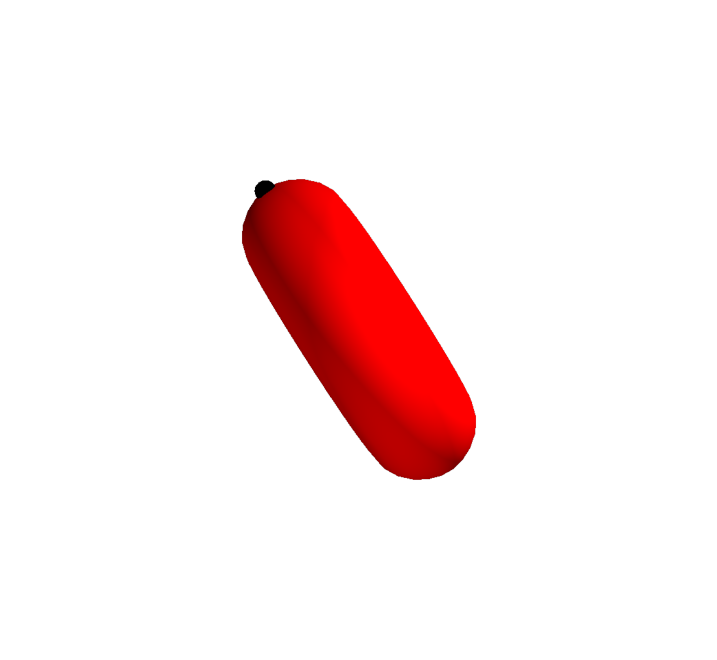
\includegraphics[trim=75 100 75 100, clip, width=\textwidth]{figures/tumble0000.png}}{0.5cm}{0.25cm}\\
        $\dot{\gamma}t = 0$
    \end{minipage}%
    \begin{minipage}{0.2\textwidth}
        \centering
        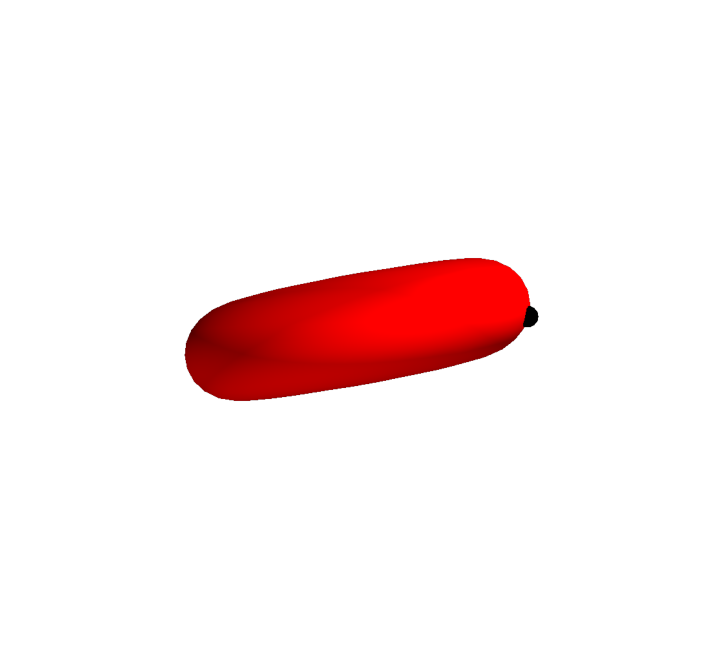
\includegraphics[trim=75 100 75 100, clip, width=\textwidth]{figures/tumble1000.png}\\
        $\dot{\gamma}t = 5$
    \end{minipage}%
    \begin{minipage}{0.2\textwidth}
        \centering
        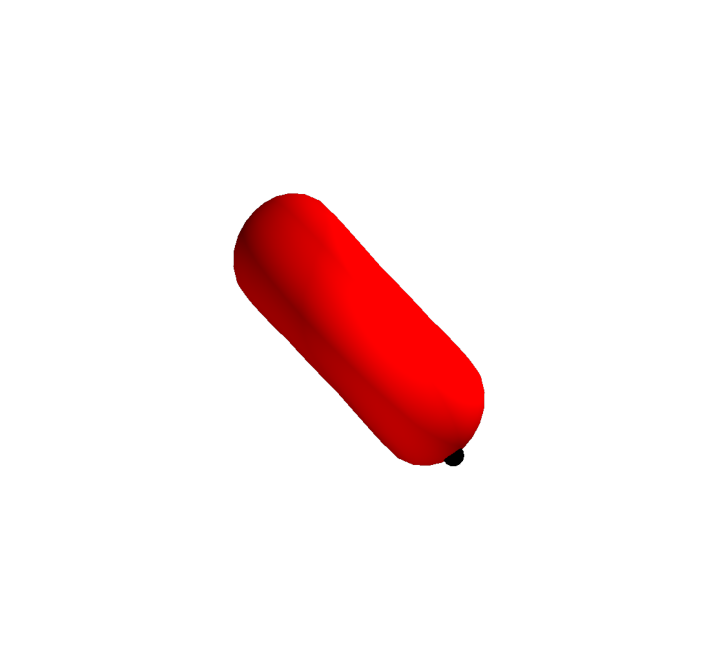
\includegraphics[trim=75 100 75 100, clip, width=\textwidth]{figures/tumble2000.png}\\
        $\dot{\gamma}t = 10$
    \end{minipage}%
    \begin{minipage}{0.2\textwidth}
        \centering
        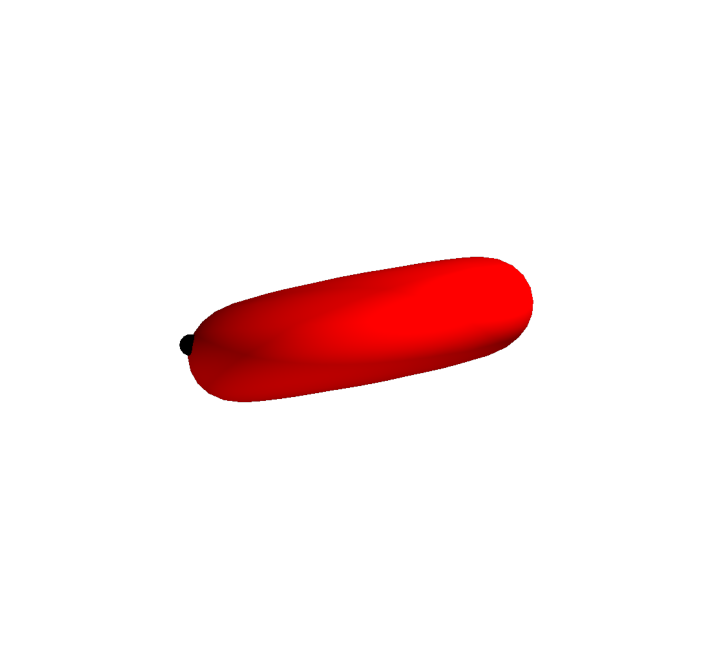
\includegraphics[trim=75 100 75 100, clip, width=\textwidth]{figures/tumble3000.png}\\
        $\dot{\gamma}t = 15$
    \end{minipage}%
    \begin{minipage}{0.2\textwidth}
        \centering
        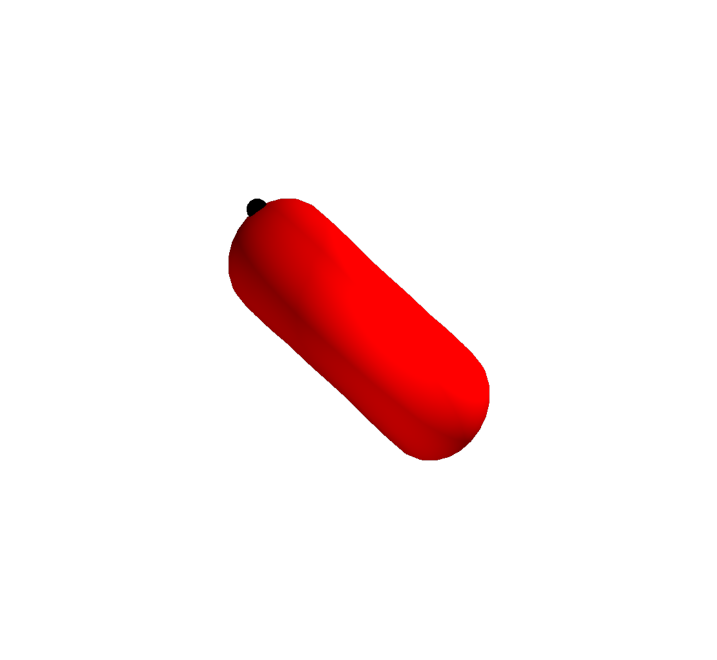
\includegraphics[trim=75 100 75 100, clip, width=\textwidth]{figures/tumble4000.png}\\
        $\dot{\gamma}t = 20$
    \end{minipage}%
    \phantomsubcaption
    \label{fig:tumble}
    \end{subfigure}
    \begin{subfigure}{\textwidth}
    \begin{minipage}{0.2\textwidth}
        \centering
        \topinset{(b)}{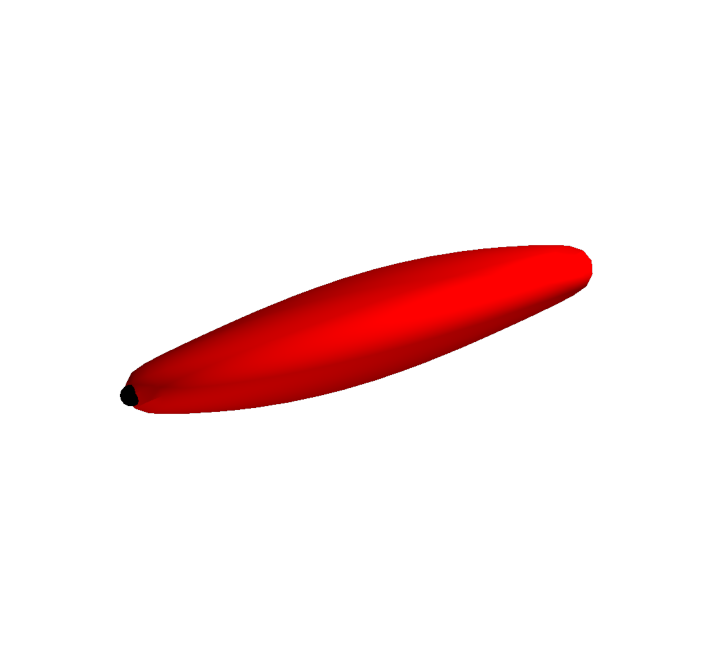
\includegraphics[trim=75 125 75 75, clip, width=\textwidth]{figures/tread0190.png}}{0.5cm}{0.25cm}\\
        $\dot{\gamma}t = 19$
    \end{minipage}%
    \begin{minipage}{0.2\textwidth}
        \centering
        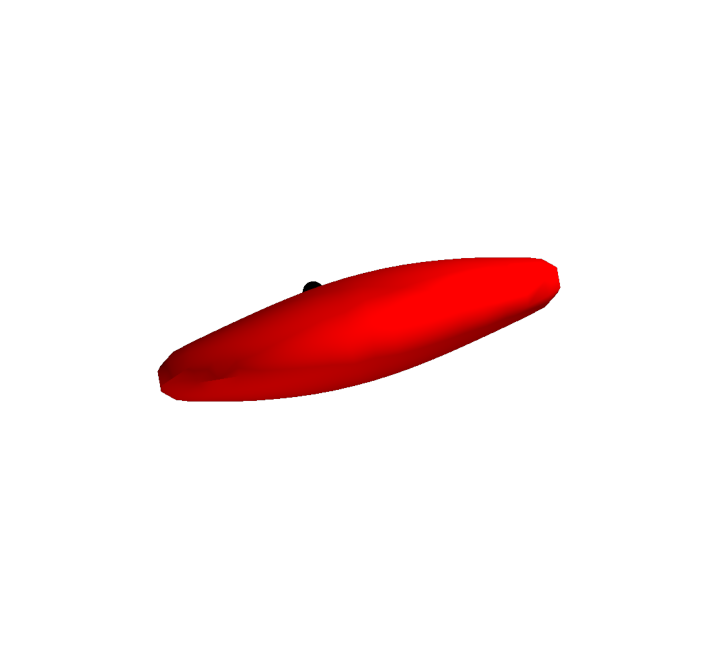
\includegraphics[trim=75 125 75 75, clip, width=\textwidth]{figures/tread0260.png}\\
        $\dot{\gamma}t = 26$
    \end{minipage}%
    \begin{minipage}{0.2\textwidth}
        \centering
        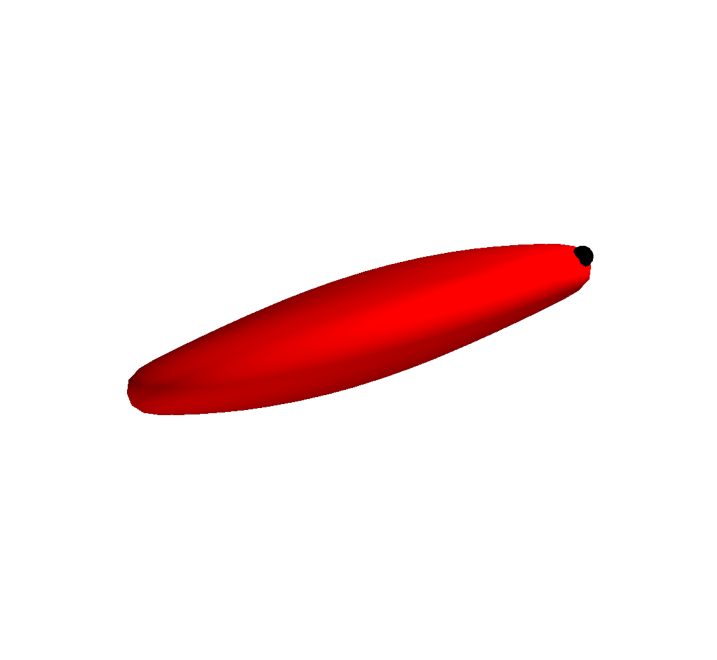
\includegraphics[trim=75 125 75 75, clip, width=\textwidth]{figures/tread0330.png}\\
        $\dot{\gamma}t = 33$
    \end{minipage}%
    \begin{minipage}{0.2\textwidth}
        \centering
        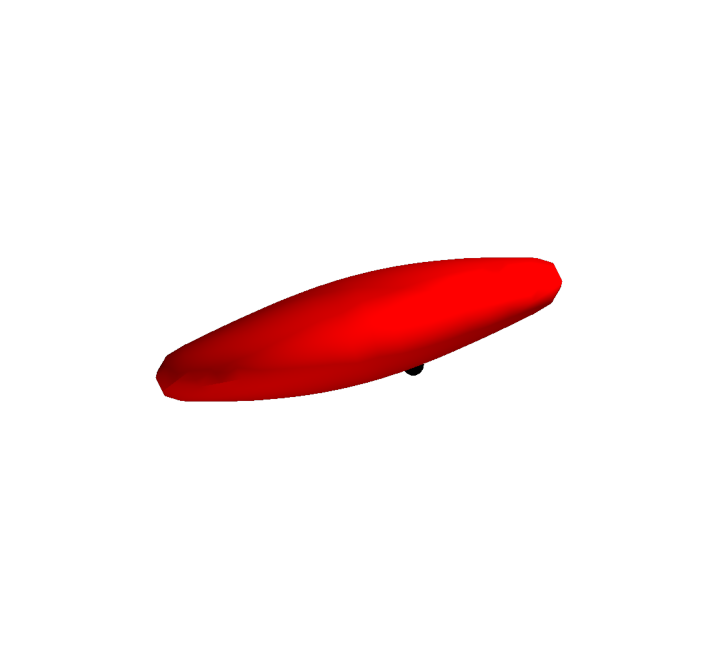
\includegraphics[trim=75 125 75 75, clip, width=\textwidth]{figures/tread0400.png}\\
        $\dot{\gamma}t = 40$
    \end{minipage}%
    \begin{minipage}{0.2\textwidth}
        \centering
        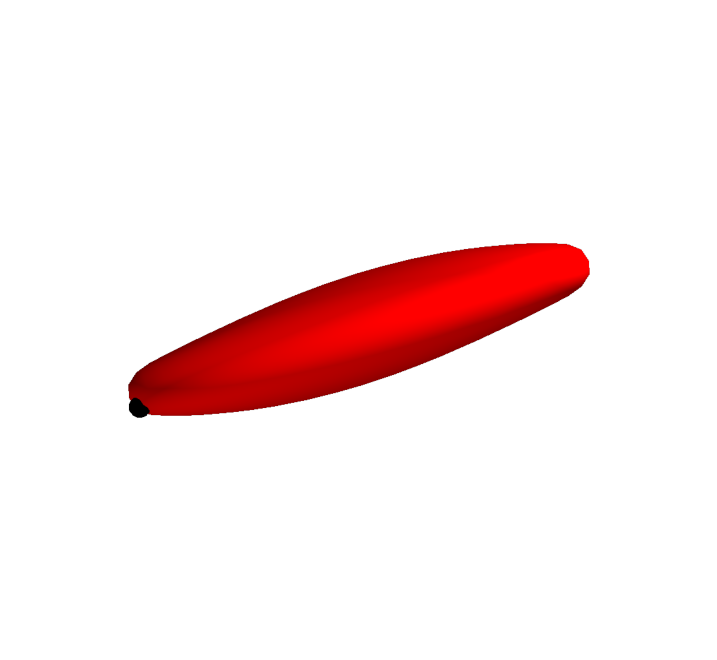
\includegraphics[trim=75 125 75 75, clip, width=\textwidth]{figures/tread0470.png}\\
        $\dot{\gamma}t = 47$
    \end{minipage}%
    \phantomsubcaption
    \label{fig:tread}
    \end{subfigure}
    \caption{%
        Our model RBC exhibits (a) a tumbling behavior under low shear
        ($\dot{\gamma} = 50\si{\per\second}$) conditions and (b) tank-treading under high
        shear ($\dot{\gamma} = 1000\si{\per\second}$) conditions.
    }%
    \label{fig:tumble-tread}
\end{figure}

%RBCs are known to tumble end-over-end under low shear conditions. As shear rates
%increase, the behavior transitions into a regime known as ``tank-treading'', in which
%the cell takes on an elongated shape and the membrane {\XXX} rotates about its interior
%fluid.
%
%We place a single RBC with $\data\cardinality = 625$ and $\sample\cardinality = 2500$
%in a $16\um\times16\um\times16\um$ domain, discretized to have $h = 0.4\um$. We use shear
%rate $\dot{\gamma} = 50\si{\per\second}$ to capture the tumbling dynamics and
%$\dot{\gamma} = 1000\si{\per\second}$ for tank-treading. One period of each is shown in
%Figure~\ref{fig:tumble-tread}.
